\documentclass[9pt,conference]{IEEEtran}
\usepackage[utf8]{inputenc}
\usepackage[brazil]{babel}

% Diversos
\usepackage{csquotes}
\usepackage{graphicx}
\usepackage{verbatim}
\usepackage{hyperref}
\usepackage{smartdiagram}

% Título
\title{Utilizando Redes Convolucionais de Grafos Espaço-Temporais para o Reconhecimento da Línguas de Sinais}
%\author{Cleison Correia de Amorim}
\date{Outubro 2018}

\author{
    \IEEEauthorblockN{Cleison Correia de Amorim}
    \IEEEauthorblockA{Centro de Informática\\
    Universidade Federal de Pernambuco\\
    Email: cca5@cin.ufpe.br}
}

% Comandos
% 'image': definição de imagem
\newcommand{\image}[4][\linewidth] {
    \begin{figure}[ht]
    \centering
    \includegraphics[width=#1]{#3}
    \caption{#4}
    \label{#2}
    \end{figure}
}

% 'refimage': referências de imagens
\newcommand{\refimage}[1] {figura \ref{#1}}

% 'refsection': referências de seções
\newcommand{\refsect}[1] {seção "\nameref{#1}"}

\begin{document}
\maketitle
\begin{abstract}
O reconhecimento de sinais é uma área de pesquisa cercada por desafios, mas que possui um papel importante para facilitar a comunicação do Surdo e para promover a remoção de barreiras ainda existentes nessa comunicação para com a sociedade. Este trabalho propõe a utilização de um modelo de aprendizagem profunda de reconhecimento de ações conhecido como Rede Convolucional de Grafos Espaço-Temporais para o contexto da língua de sinais. Trata-se de uma nova abordagem centrada no movimento do esqueleto humano que utiliza grafos para capturar o movimento do corpo sob duas dimensões: espacial e temporal, e que é capaz de considerar aspectos desafiadores da dinâmica dessa língua. Além disso, este trabalho também apresenta a criação de um novo \textit{dataset} de esqueletos humanos para a língua de sinais americana baseado no ASLLVD, o qual é utilizado com o modelo acima e disponibilizado com o intuito de contribuir com a evolução de estudos relacionados a essa área.
\end{abstract}

\begin{IEEEkeywords}
Língua de Sinais, Redes Neurais Convolucionais, Grafos Espaço-Temporais.
\end{IEEEkeywords}


\section{Introdução} %%%%%%%%%%%%%%%%%%%%%%%%%%%%%%%%%%%%%%%%%%%
\label{sec:introducao}

A língua de sinais é uma ferramenta de comunicação visual e que possibilita com que indivíduos que possuem diferentes tipos de deficiência auditiva se comuniquem entre si e com os demais indivíduos na comunidade. Ela é a língua utilizada pela maioria dos Surdos em sua vida diária e, muito além do que isso, ela é o símbolo de identificação entre os membros dessa comunidade e também a principal força que os une \cite{pereira-choi-2011}. 

%Sign language is a language that provides visual communication and allows individuals with hearing or speech impairments to communicate with each other or with other individuals in the community. 
%Segundo Pereira, Choi, et al. (2012), hoje a língua de sinais é a língua usada pela maioria dos Surdos em sua vida diária. É o símbolo de identificação entre os membros da comunidade Surda e também a principal força que os une. 

Assim como nas línguas orais, existe uma relação muito estreita entre essa língua e a cultura dos diferentes países onde são utilizadas. Por esse motivo, apesar de compartilharem diversos traços em comum e de muitas vezes ser fácil transitar entre elas, cada país possui uma língua de sinais própria nascida e desenvolvida com as suas comunidades Surdas \cite{pereira-choi-2011}.

%Essa língua não é universal e cada país tem a sua, da mesma forma como eles possuem uma língua na modalidade oral. Há uma relação muito estreita entra a língua e cultura: as línguas de sinais refletem a cultura dos diferentes países onde são utilizadas e nasceram junto com as suas comunidades Surdas. Por esse motivo elas também são consideradas línguas naturais, segundo os autores.

Segundo a Organização Mundial de Saúde, hoje o número de pessoas com deficiência auditiva incapacitante é de cerca de 466 milhões e estima-se que até 2050 esse número ultrapasse os 900 milhões -- o que equivale a uma proporção global de 1 em cada 10 indivíduos \cite{who-2018}. Esses dados ressaltam a abrangência e a importância do papel das línguas de sinais para viabilizar a comunicação das pessoas ao redor do mundo. 

%According to the World Health Organization, the number of hearing-impaired individuals has recently reached 400 million. For this reason, recent studies have been accelerated to make disabled people communicate more easily.


Apesar disso, é muito pequeno o número de pessoas ouvintes que são capazes de se comunicar utilizando a língua de sinais. Isso acaba caracterizando uma barreira invisível que interfere na comunicação entre as comunidades Surda e ouvinte, inviabilizando uma integração mais efetiva entre elas \cite{peres-2006}. Nesse contexto, faz-se necessário no âmbito da tecnologia desenvolver ferramentas que sejam capazes de preencher essa lacuna e promover a inclusão entre essas pessoas. 

%Apesar das conquistas que a comunidade Surda tem alcançado nos últimos anos, entre as quais o reconhecimento da importância das línguas de sinais na comunicação é certamente a mais notável, essa língua ainda não se disseminou o suficiente entre as pessoas que não têm contato direto com tal comunidade. Isso acaba caracterizando uma barreira invisível que interfere na comunicação entre as comunidades Surda e ouvinte, inviabilizando uma interação e inclusão mais efetiva entre ambas (PERES, FLORES, et al., 2006).

%Very few hearing people are able to communicate in sign language. Therefore, there is a need to develop a recognition system to bridge the communication gap between the hearing and hearing impaired communities. For that reason, the sign language recognition problem has been researched since 1990s. A sign is not only performed with hand motion and hand shapes (manual components), but also through facial expressions, head motion and body postures (non-manual components).

Por essa razão, estudos relacionados com o reconhecimento da língua de sinais vêm sendo desenvolvidos desde a década de 1990 e é possível constatar resultados significativos a partir deles \cite{lim-2016, recent-advances-dl-2017}. Os principais desafios encontrados por eles estão relacionados primeiramente com considerar os aspectos dinâmicos da língua, como por exemplo os movimentos, articulações entre partes do corpo e as expressões não-manuais, ao invés de limitarem-se a apenas reconhecer sinais estáticos ou posições de mãos isoladas. Além disso, a língua de sinais apresenta milhares de sinais, que às vezes diferem-se apenas por mudanças sutis no movimento, forma ou posição da mão e envolvem sobreposições significativas de dedos e oclusões. Quando combinadas as diferenças no estilo de sinalização entre indivíduos, bem como as variações no estilo decorrentes da não-universalidade ou de regionalismos da língua, essa linha de pesquisa pode se tornar ser muito desafiadora para os atuais algoritmos de inteligência computacional \cite{konstantinidis-2018}.

% This is due to the fact that sign language features thousands of signs, sometimes differing only by subtle changes in hand motion, shape or position and involving significant finger overlaps and occlusions. Combined also with differences in the signing style between individuals, SLR can be very challenging for current computer vision algorithms. 
% Isto se deve ao fato de que a linguagem de sinais apresenta milhares de sinais, às vezes diferindo apenas por mudanças sutis no movimento, forma ou posição da mão e envolvendo sobreposições significativas de dedos e oclusões. Combinado também com diferenças no estilo de assinatura entre indivíduos, o SLR pode ser muito desafiador para os atuais algoritmos de visão computacional
% Finally, the unavailability of large sign language datasets and the fact that sign language is not universal but presents significant variations based on the ethnicity of signers pose challenges to the development of an accurate and robust SLR system.

Dessa forma, este trabalho apresenta a aplicação ao reconhecimento da língua de sinais de uma nova abordagem capaz de realizar o reconhecimento de ações humanas tomando como base grafos espaço-temporais, a qual é denominada Redes Convolucionais de Grafos Espaço Temporais (ou \textit{Spatial-Temporal Graph Convolutional Networks} - ST-GCN) \cite{st-gcn-2018}.
Ao utilizar representações em grafos do esqueleto humano, essa abordagem centraliza seu foco no movimento desse corpo e nas interações entre suas partes, desconsiderando a interação com o ambiente à sua volta. Além disso, ela também aborda os movimentos dos indivíduos sob duas dimensões distintas, a espacial e e temporal, o que lhe faz capaz de capturar os aspectos dinâmicos das ações exercidas. Essas características fazem dessa uma abordagem relevante para lidar com os desafios da língua de sinais aqui apresentados e justificam, portanto, sua adoção aqui.

Entretanto, para que fosse possível utilizar o ST-GCN nesse contexto, foi necessário primeiro desenvolver um \textit{dataset} de esqueletos humanos da língua de sinais que serviria como a informação principal para alimentar esse modelo. Para isso, foi utilizado como base o \textit{American Sign Language Lexicon Video Dataset} (ASLLVD), que consiste numa ampla base de sinais da língua americana, a partir dos quais foram estimados e extraídos os esqueletos necessários para o novo \textit{dataset}.

Sendo assim, este trabalho traz como principais contribuições: 1) a adoção de uma nova técnica centrada no movimento humano para o reconhecimento de sinais, a qual é capaz de considerar diferentes aspectos da dinâmica da língua sinalizada e ajudar a contornar alguns desafios apresentados acima nessa direção; 2) a criação e disponibilização\footnote{
    Disponível em \url{http://www.cin.ufpe.br/~cca5/asllvd-poses}
} de um \textit{dataset} de esqueletos humanos para a língua de sinais americana, o qual objetiva contribuir com a evolução de estudos futuros em áreas correlatas.

Este trabalho está organizado da seguinte forma: na \refsect{sec:trabalhos-relacionados} são apresentados os trabalhos relacionados e o funcionamento do ST-GCN em maiores detalhes; a \refsect{sec:experimentos} aborda a condução dos experimentos, incluindo o processo de criação do \textit{dataset} acima e os ajustes realizados no ST-GCN para o reconhecimento da língua de sinais; por fim, na seção \refsect{sec:resultados} estão contidos os resultados obtidos a partir da abordagem aplicada.



\section{Trabalhos Relacionados} %%%%%%%%%%%%%%%%%%%%%%%%%%%%%%%%%%%%%%%%%%%%%%%%%%%%%%%%%%%%%%%%%%%%
\label{sec:trabalhos-relacionados}

O reconhecimento de línguas de sinais tem apresentado progressos relevantes nos últimos anos, os quais são motivados principalmente pelo advento de sensores mais modernos, de novas técnicas de aprendizagem de máquina e de \textit{hardwares} mais potentes que viabilizam o surgimento de algoritmos ainda mais robustos \cite{recent-advances-dl-2017, recent-advances-sl-2013}. Além disso, técnicas consideradas intrusivas e requerem a utilização de sensores como luvas, acelerômetros e marcadores acoplados ao corpo do interlocutor para captura dos sinais vêm sendo abandonadas, e cedendo espaço para abordagens baseadas em câmeras e visão computacional.

Para isso, também tem crescido a adoção de técnicas de extração de características como SIFT \cite{sift-2004}, HOG \cite{hog-2005}, HOF \cite{hof-2008} e STIP \cite{hof-2008} \cite{recent-advances-dl-2017} afim de pré-processar as imagens capturadas por essas câmeras e fornecer informações mais ricas para utilização em conjunto com algoritmos de aprendizagem de máquina \cite{lim-2016, shanta-2018}.

Nessa linha, em \cite{lim-2016} foi introduzida uma abordagem de Histograma de Fluxo Óptico Baseado em Blocos de representação (ou \textit{Block-Based Histogram of Optical Flow} - BHOF) para o reconhecimento da linguagem de sinais a partir das imagens das mãos. Nele, primeiramente a face do signatário é rastreada e removida, e o modelo de segundo plano é construído por meio da fusão dos filtros mediano e de moda em toda a sequência de vídeo para detectar as mãos. Com base nesse modelo de segundo plano, o primeiro plano é então extraído e a posição da mão é determinada. Em seguida, as regiões do fluxo óptico das mãos são extraídas e o fluxo óptico do histograma baseado em blocos é finalmente calculado e utilizado na classificação. 

Nos últimos anos, é possível também perceber uma presença notável da utilização de Redes Neurais Convolucionais (ou CNNs) na resolução do problema do reconhecimento das línguas de sinais. Sua utilização para o reconhecimento de línguas de diferentes nacionalidades têm sido capaz de demonstrar resultados favoráveis, com acurácia comumente superior a 90\%  \cite{shanta-2018, ji-2017, taskiran-2018, rao-2018}. Algumas variações também são encontradas com esse mesmo propósito, como o uso de 3D CNNs \cite{elbadawy-2017}, combinada com o modelo Inception \cite{das-2018} ou com o uso de Regiões de Interesse \cite{sajanraj-2018}. Além das CNNs, pode-se também constatar, em menor proporção, a adoção de Redes Neurais Recorrentes \cite{konstantinidis-2018} e de Redes Residuais Temporais \cite{pigou-2017} para o reconhecimento de sinais.

Apesar desses avanços, muitos desses estudos ainda restringe-se a adotar apenas imagens estáticas dos sinais ou de letras isoladas da datilologia\footnote{
     Datilologia – também conhecida como alfabeto digital ou alfabeto manual. Consiste na soletração de palavras pelos Surdos. É geralmente utilizada para introduzir uma palavra que ainda não possui um sinal equivalente \cite{quadros-2004, pereira-choi-2011}.
} \cite{shanta-2018, taskiran-2018, elbadawy-2017, das-2018, sajanraj-2018}. Isso torna-se um ponto negativo quando observamos pela dimensão de que essa abordagem desconsidera o aspecto dinâmico da língua que é intrínseco ao cotidiano do Surdo, como seus movimentos, expressões não-manuais e articulações entre partes do corpo \cite{quadros-2004}. Dessa forma, faz-se extremamente relevante desenvolver técnicas capazes de considerar a dinâmica da língua de sinais como em \cite{konstantinidis-2018} e \cite{pigou-2017}. 

Com esse propósito, este trabalho aplica uma abordagem de reconhecimento de ações por meio do esqueleto humano denominada de Rede Convolucional de Grafos Espaço-Temporais (ou \textit{Spatial-Temporal Graph Convolutional Network - ST-GCN}) apresentada em \cite{st-gcn-2018} para o problema do reconhecimento da língua de sinais. 

A motivação da ST-GCN surgiu a partir da necessidade enxergada pelos autores de métodos que fossem capazes de capturar de forma autônoma os padrões contidos na configuração espacial das articulações do corpo humano, bem como sua dinâmica temporal. Segundo eles, os métodos anteriores de uso de esqueletos para reconhecimento de ações eram limitados justamente por não explorar explicitamente tais relações espaciais entre as articulações, que são cruciais para a compreensão das ações humanas. Esses métodos, simplesmente empregaram as coordenadas conjuntas em etapas de tempo individuais para formar vetores de característica, aplicando uma análise temporal neles \cite{st-gcn-2018, wang-2012, fernando-2015}.

Mais recentemente, eles afirmam, novos métodos que tentaram alavancar as conexões naturais entre as articulações foram desenvolvidos \cite{shahroudy-2016, yong-du-2015}. Eles mostraram melhorias encorajadoras, o que sugere a importância da conectividade. No entanto, a maioria desses métodos baseia-se em partes ou regras criadas manualmente para analisar os padrões espaciais. Como resultado, os modelos criados para uma aplicação específica são difíceis de serem generalizados para outras \cite{st-gcn-2018}.

O ST-GCN, por sua vez, tem como base de sua formulação uma sequência de grafos de esqueletos que representam o corpo humano, os quais são obtidos a partir de uma série de \textit{frames} de vídeos de ações ordinárias desses indivíduos. A \refimage{fig:st-gcn-graph} permite-nos visualizar essa estrutura, onde cada nó corresponde a um ponto de articulação humana. Os vértices intra-corporais são definidos com base nas conexões naturais do corpo. Os vértices inter-frames, por sua vez, conectam as mesmas articulações entre \textit{frames} consecutivos para denotar sua trajetória no decorrer do tempo \cite{st-gcn-2018}.

\image
	[4cm]
    {fig:st-gcn-graph}
    {images/st_gcn_graph}
    {Sequência de grafos de esqueletos, que denotam o movimento humano no espaço e no tempo, utilizados pelo ST-GCN. Fonte: \cite[p. 1]{st-gcn-2018}.}

A \refimage{fig:st-gcn-workflow} ilustra a abordagem utilizada pelo ST-GCN. Nela, primeiro é realizada a estimação das poses dos indivíduos nos vídeos de entrada e a construção de grafos espaço-temporais com base nessa sequência de esqueletos estimados. Em seguida, múltiplas camadas de convolução ST-GCN são aplicadas gerando, gradualmente, mapas de características de nível cada vez mais alto para os grafos apresentados. Por fim, eles são submetidos a um classificador para a identificação da ação correspondente.

\image
    {fig:st-gcn-workflow}
    {images/st_gcn_workflow}
    {Fluxo do ST-GCN, onde os grafos criados a partir dos indivíduos presentes nos vídeos são submetidos ao modelo e, por fim, classificados entre as ações disponíveis. Fonte: \cite[p. 3]{st-gcn-2018}.}


% Funcionamento do ST-GCN ------------------------

Para que seja possível compreender o funcionamento da rede ST-GCN em detalhe, é necessário primeiro aprofundarmos a discussão nas estratégias de amostragem e de particionamento adotadas por ele. 

É fácil visualizar a existência de um \textit{grid} rígido ou retângulo em volta de um ponto central quando lidamos com convoluções em imagens 2D. o qual delimita a vizinhança na qual o filtro convolucional será aplicado. No caso dos grafos, entretanto, é necessário ir além dessa definição e considerar que a vizinhança de um ponto será composta apenas por aqueles pontos que estão diretamente conectados a ele por meio de um vértice. A \refimage{fig:st-gcn-sampling} permite-nos visualizar essa definição para o exemplo de um único \textit{frame}. Observe que as bordas tracejadas vermelhas passam a representar a área de amostragem utilizada pelo filtro convolucional, em volta dos pontos vermelho. Observe também que, apesar de haver pontos do corpo localizados próximos fisicamente no espaço (como no caso dos pontos dos pés, joelhos e cintura), eles não serão considerados como vizinhos na abordagem de convolução em grafos por não possuírem conexões diretas entre si.

\image
	[3cm]
    {fig:st-gcn-sampling}
    {images/st_gcn_sampling}
    {\textit{Frame} de exemplo de um esqueleto de entrada. As articulações do corpo são desenhadas com pontos azuis. Os pontos vermelhos representam os pontos centrais de um filtro com distância D = 1 aplicado ao \textit{frame}, cuja abrangência é delimitada pela linha tracejada vermelha. Fonte: \cite[p. 5]{st-gcn-2018}.}

Por meio da \refimage{fig:st-gcn-sampling} é possível observar que apenas estão sendo considerados pela linha tracejada os pontos que estão imediatamente conectados aos pontos centrais. Em outras palavras, diz-se que a área de \textbf{amostragem} do filtro convolucional apenas considera vizinhos com distância D = 1. Essa distância poderia ser ajustada para abranger vizinhos mais distantes, porém na apresentação do ST-GCN \cite{st-gcn-2018} os autores estabeleceram a utilização da distância conforme acima.

Uma vez apresentada a amostragem, é possível seguir na compreensão da estratégia de \textbf{particionamento}, que é definida como Particionamento de Configuração Espacial. Ela está baseada na localização das partes e nas características do movimento do corpo humano, conforme ilustra a \refimage{fig:st-gcn-spatial-part}.

\image
	[3cm]
    {fig:st-gcn-spatial-part}
    {images/st_gcn_spatial_partitioning}
    {Particionamento de Configuração Espacial: os nós são rotulados de acordo com suas distâncias ao centro de gravidade do esqueleto (cruz preta) comparado com o do nó raiz (verde). Os nós centrípetos têm distâncias menores (azul), enquanto os nós centrífugos têm distâncias mais longas (amarelo) do que o nó raiz. Fonte: \cite[p. 5]{st-gcn-2018}.}

De acordo com os autores, a estratégia desenvolvida motiva-se no fato de que os movimentos das partes do corpo podem ser amplamente categorizados como concêntricos ou excêntricos e, por isso, os pontos na região de amostragem são particionados em três subconjuntos:

\begin{enumerate}
    \item O nó raiz (ou ponto central, sinalizado em verde na imagem);
    \item O grupo centripetal (pontos em azul na imagem): nós da vizinhança que estão mais próximos do centro de gravidade do esqueleto (cruz preta na imagem) do que o nó raiz;
    \item O grupo centrifugal (pontos em amarelo na imagem): mais distante do centro de gravidade do que o nó raiz;
\end{enumerate}

O centro de gravidade é definido como sendo a coordenada média de todas as juntas do esqueleto em um \textit{frame}. Durante a convolução, cada ponto do corpo é rotulado segundo uma das partições acima.

O ST-GCN define uma estratégia de atribuição de pesos que também é direcionada por essas partições e, para cada uma delas, recebe um peso distinto. Em outras palavras, ao invés de concentrar sua atenção no movimento das juntas do corpo de forma individual, ele direciona seu foco a aprender o tipo do movimento realizado por essas juntas.

Uma vez exploradas as estratégias definidas pelo ST-GCN, apresentadas sob o contexto de um único \textit{frame} na dimensão espacial, é possível aprofudar essa discussão para compreender como o modelo considera a dimensão temporal. 

Retomemos à definição inicial que estabelece que a dimensão temporal é formada por uma sequência de grafos de esqueletos extraídos dos \textit{frames} de vídeo de uma ação, conforme \refimage{fig:st-gcn-graph}. Se selecionássemos um desses grafos, constataríamos que ele possui dois vizinhos: o grafo imediatamente anterior e aquele imediatamente posterior a ele na sequência. Além disso, foi definido também que cada articulação deve estar conectada a ela mesma nos grafos vizinhos afim de representar sua evolução no tempo. Nesse ponto já seríamos capazes de evoluir a compreensão de amostragem espacial também para a dimensão temporal, se considerarmos que o ponto central em vermelho da \refimage{fig:st-gcn-graph}, além dos pontos delimitados pela linha tracejada vermelha, agora passará a ter como vizinhos também aqueles pontos com os quais está conectado nos seus vizinhos anterior e posterior da sequência. Dessa forma, a linha tracejada vermelha passaria a englobar também aqueles pontos diretamente conectados e dispostos na dimensão temporal, conforme ilustrado na \refimage{fig:st-gcn-convolution} (à esquerda).

\image
	[9cm]
    {fig:st-gcn-convolution}
    {images/st_gcn_convolution}
    {Amostragem englobando pontos diretamente conectados nas dimensões espacial e temporal (à esquerda) e processo de convolução espaço-temporal sob os pontos da amostragem obtida (ao centro e à direita).  Fonte: \cite[p. 3]{st-gcn-2018}.}

Uma vez realizada a amostragem sob as duas dimensões e selecionados os pontos para a convolução, é possível aplicar esse processo de uma forma análoga àquela aplicada a imagens 2D, conforme ilustra a \refimage{fig:st-gcn-convolution} (ao centro e à direita).


% Arquitetura ------------------------

A \refimage{fig:st-gcn-architecture} (à esquerda) permite-nos visualizar as camadas de convolução do modelo. Ao todo, são nove camadas convolucionais ST-GCN posicionadas de forma sequencial, que realizam a extração das características dos grafos espaço-temporais apresentados. Elas são precedidas por uma camada de normalização e seguidas por uma camada de \textit{pooling} global e outra de classificação \textit{softmax}. À direita da imagem é apresentado também o detalhe de uma unidade convolucional ST-GCN.

\begin{figure}[ht]
    \centering
    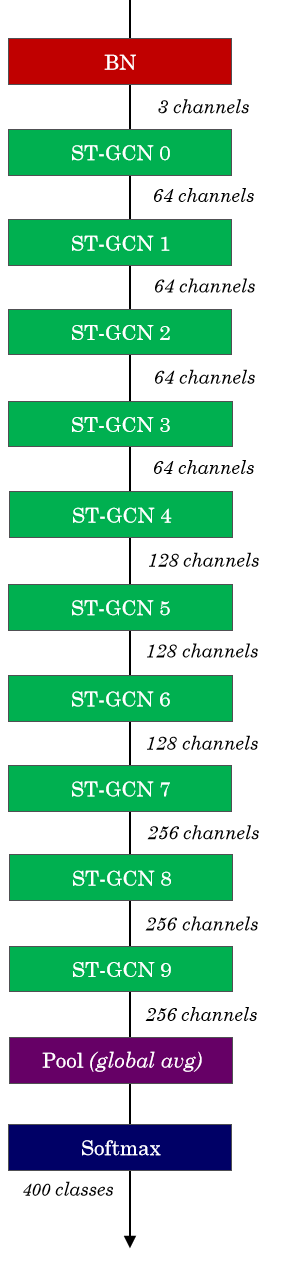
\includegraphics[width=3.0cm]{images/st_gcn_architecture}
    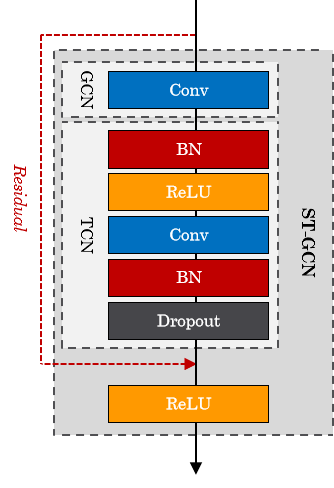
\includegraphics[width=3.5cm]{images/st_gcn_architeture_unit}
    \caption{Arquitetura do modelo (à esquerda) e detalhe de uma unidade ST-GCN (à direita). Unidades de ST-GCN aplicam operações de normalização, convolução, ativação e \textit{dropout} aos grafos e levam em consideração o valor residual da camada anterior para calcular as ativações de saída. Fonte: adaptado de \cite{st-gcn-2018}.}
    \label{fig:st-gcn-architecture}
\end{figure}


Para que fosse possível realizar a estimação das poses dos indivíduos, conforme fluxo da \refimage{fig:st-gcn-workflow}, os autores utilizaram uma biblioteca denominada OpenPose. Trata-se de uma ferramenta que utiliza algoritmos de aprendizagem profunda para detectar indivíduos em cenas de vídeos e extrair até 135 pontos de articulações de seus corpos, mãos e faces \cite{cao-realtime-2017, simon-hand-2017, wei-cpm-2016}, e que está disponível publicamente\footnote{
    Disponível em \url{https://github.com/CMU-Perceptual-Computing-Lab/openpose}.
}.

Na apresentação do ST-GCN, entretanto, os autores utilizaram apenas 18 desses pontos, os quais se referem às articulações do corpo (vide \refimage{fig:keypoints-pose}). O código fonte e os modelos pré-treinados do ST-GCN estão disponíveis publicamente pelos autores\footnote{
    Disponível em \url{https://github.com/yysijie/st-gcn}.
}.

\image
	[4cm]
    {fig:keypoints-pose}
    {images/keypoints_pose_COCO_18}
    {Representação dos 18 pontos referentes ao corpo humano, extraídos pelo OpenPose. Fonte: \cite{openpose-output-2018}.}

Todo o fluxo descrito até aqui trata da aplicação do ST-GCN para o contexto onde vídeos isolados são gravados previamente e utilizados como entrada. Apesar disso, entende-se que seria possível, com algum trabalho adicional, evoluí-lo na direção de substituir essa entrada por um \textit{streaming} de vídeo capturado em tempo real por uma câmera. Para isso, seria necessário passar a estimar continuamente com uma biblioteca ou \textit{hardware} específico as poses dos \textit{frames} capturados, provendo assim um \textit{streaming} de esqueletos para o modelo. A biblioteca OpenPose (que está descrita em detalhes mais adiante) é capaz de atender a essa necessidade, porém seus requisitos de \textit{hardware} robusto podem acabar por limitar sua adoção em alguns contextos na prática. A leitura dos dados pelo modelo também precisaria ser evoluída afim de que ao invés de considerar informações em arquivos físicos, sejam utilizadas aquelas fornecidas pelo \textit{streaming} de esqueletos. Como o ST-GCN hoje só trabalha com vídeos de tamanho fixo, essa entrada em fluxo contínuo apenas seria classificada por ele de janelas em janelas de tempo, quando completado em memória esse número fixo estabelecido de \textit{frames}.


\section{Experimentos} %%%%%%%%%%%%%%%%%%%%%%%%%%%%%%%%%%%%%%%%%%%%%%%%%%%%%%%%%%%%%%%%%%%%%%%
\label{sec:experimentos}

A pesquisa foi organizada segundo passos estabelecidos abaixo. Em termos gerais, eles definem desde a identificação de um modelo em potencial conforme objetivos estabelecidos na \refsect{sec:introducao}, sua adaptação para o problema da língua de sinais até a avaliação de seu desempenho.

\begin{enumerate}
    \item Definir modelo: nesse passo foi selecionado o modelo ST-GCN e sua abordagem baseada em grafos para lidar com o problema da língua de sinais;
    \item Definir \textit{dataset}: foi estabelecido o ASLLVD, devido à sua abrangência relevante de sinais, qualidade das amostras coletadas, organização das anotações e rotulações, e articulação dos sinais por indivíduos nativos. Apesar de baseado na Língua Americana de Sinais, a utilização desse \textit{dataset} não restringe a abordagem apresentada à língua daquele país. Ao contrário, entende-se que é possível adotar o mesmo método a \textit{datasets} de línguas de outros países;
    \item Preparar \textit{dataset}: para que fosse possível utilizar o \textit{dataset} acima com o ST-GCN foi necessário primeiro criar um \textit{pipeline} de pré-processamento, conforme descrito mais adiante nesta seção, afim de colocar cada amostra em  um formato compatível com a entrada do modelo;
    \item Adaptar modelo: para que fosse possível utilizar o ST-GCN no contexto da língua de sinais, foi necessário realizar pequenas adaptações na interpretação dos grafos e na leitura dos dados. Esse processo também está melhor descrito mais adiante;
    \item Treinar modelo adaptado: nesse passo, o modelo acima será submetido às amostras do \textit{dataset} para que possa desenvolver um conhecimento acerca do problema;
    \item Avaliar e melhorar resultados: a partir das descobertas obtidas na tarefa acima, serão realizados os eventuais ajustes no modelo, \textit{dataset} ou nas configurações do treinamento, e repetido o passo anterior.
\end{enumerate}


\subsection{Dataset} %%%%%%%%%%%%%%%%%%%%%%%%%%%%%%%%%%%%%%%%%%%%%%%%%%%%%%%%%%%%%%%%%%%%%%%%%%%%%%%%%

O \textit{American Sign Language Lexicon Video Dataset} (ou ASLLVD) consiste num \textit{dataset} público\footnote{
    Disponível em \url{http://csr.bu.edu/asl/asllvd/annotate/index.html}.
} amplo e em expansão que contém sequências de vídeos de milhares de sinais distintos da Língua Americana de Sinais (\textit{American Sign Language}, ou ASL), bem como as anotações dessas sequências, os \textit{frames} de início e fim, e os rótulos de classe para cada sinal \cite{athitsos-asllvd-2008, neidle-2012, vloger-2012}.

Segundo os autores, cada sinal é articulado por indivíduos nativos da ASL, e as sequências de vídeo são coletadas utilizando um sistema de quatro câmeras que captura simultaneamente duas vistas frontais, uma vista lateral e uma vista ampliada na face desses indivíduos. A \refimage{fig:asllvd-example} exemplifica a captura de três dessas vistas para o sinal "\textit{MERRY-GO-ROUND}".

\image
    {fig:asllvd-example}
    {images/asllvd_example}
    {Exemplo de captura do sinal \textit{"MERRY-GO-ROUND"} sob três perspectivas, no ASLLVD. Fonte:  \cite[p. 2]{athitsos-asllvd-2008}.}

Ainda de acordo com os autores, o número e o tipo de sinais incluídos no ASLLVD são semelhantes em escala e escopo ao conjunto de entradas lexicais nos dicionários existentes de "Inglês-para-ASL". Existe ao menos um exemplo de vídeo por sinal (articulado por um indivíduo nativo), para quase todos os sinais contidos no Dicionário Gallaudet de Língua Americana de Sinais \cite{athitsos-asllvd-2008, gallaudet-2005}. 

Ao analisar os metadados do \textit{dataset} é possível identificar a existência de um total de 2.745 sinais, representados em 9.757 amostras. Cada sinal contém entre 1 e 18 amostras articuladas por diferentes indivíduos (sendo 4 o número médio de amostras por sinal).
%%%%%%%%%%%%%%%%%%%%%%%%%%%%%%%%%%%%%%%%%%%%%%%%%%%%%%%%%%%%%%%%%%%%%%%%%%%%%%%%%%%%%%%%%%%%%%%%%%%%%%%%%%%%%%%%%%%%

\subsection{Pré-processamento do Dataset} %%%%%%%%%%%%%%%%%%%%%%%%%%%%%%%%%%%%%%%%%%%%%%%%%%%%%%%%%%%%%%%%%%%%%%%%%%%
\label{sec:preproc-dataset}

Para tornar as amostras do ASLLVD compatíveis com a entrada esperada pelo modelo ST-GCN foram aplicadas várias etapas de pré-processamento em série, as quais estão apresentadas na \refimage{fig:preprocessamento} e definidas em detalhe a seguir.

%\begin{figure}[ht]
%    \centering
%    \smartdiagramset{
%        border color=none,
%        back arrow disabled=true,
%        text width=1cm}
%    \smartdiagram[sequence diagram]{
%        Obter vídeos,
%        Segmentar amostras,
%        Estimar poses, 
%        Holdout, 
%        Processar amostras}
%    \caption{Etapas de pré-processamento aplicadas ao \textit{dataset} ASLLVD.}
%    \label{fig:preprocessamento}
%\end{figure}

\image
    {fig:preprocessamento}
    {images/dataset_preprocessing}
    {Etapas de pré-processamento aplicadas ao \textit{dataset} ASLLVD.}

A primeira delas consiste num passo preliminar de \textbf{obtenção dos vídeos} que compõem o \textit{dataset} a partir das URLs onde estão disponibilizados, afim de reconstituir a base localmente de forma automática, viabilizando as etapas posteriores. A relação das vídeos e respectivas seções contidas no ASLLVD foi utilizada para guiar esse processo está disponibilizada juntamente com ele em um arquivo de metadados específico\footnote{
    Disponível em \url{http://www.bu.edu/asllrp/dai-asllvd-BU_glossing_with_variations_HS_information-extended-urls-RU.xls}
}. Apesar do \textit{dataset} conter capturas de até 4 câmeras distintas para um mesmo sinal, este trabalho considera apenas a captura realizada pela câmera frontal, que contempla os movimentos do tronco, mãos e face, simultaneamente.

A etapa seguinte consiste em \textbf{segmentar os vídeos} obtidos acima em vídeos individuais por sinal, uma vez que cada arquivo original corresponde a uma seção onde foram gravados múltiplos sinais por indivíduo. O intuito dessa tarefa é constituir um novo conjunto organizado de forma tal que cada sinal esteja disposto de forma individual com seu respectivo rótulo. Para isso, também foi considerado o arquivo de metadados comentado acima, que dispõe dos rótulos aqui requeridos e das respectivas marcações de \textit{frames} de início e término para cada sinal dentro das seções. Como saída dessa etapa, são obtidos vídeos com duração média de 1 a 5 segundos e com aspecto semelhante ao que se observa na \refimage{fig:sign-original}.

\image
    [5cm]
    {fig:sign-original}
    {images/sign_original}
    {Representação do sinal "EXAGGERATE", segmentado a partir das seções gravadas para o ASLLVD. Fonte: \cite{athitsos-asllvd-2008}.}

O terceiro passo consiste em realizar a \textbf{estimação das poses} dos indivíduos presentes em cada um dos vídeos segmentados. Em outras palavras, isso significa extrair as coordenadas das partes do corpo desses indivíduos, \textit{frame} a \textit{frame}, para compor os esqueletos que são a base dos grafos que serão utilizados pelo modelo. Para isso, utilizou-se a biblioteca OpenPose, que é a mesma adotada pelos autores em \cite{st-gcn-2018}. A diferença, entretanto, está no fato de que além das coordenadas referentes ao corpo dos atores, um número consideravelmente maior de coordenadas foi necessário para que fosse possível abranger também as mãos e face dos indivíduos. No total são 130 pontos, dos quais 21 correspondem a cada uma das mãos; 70 correspondem às coordenadas da face; e 18 correspondem aos pontos corpo (vide \refimage{fig:keypoints-face-hand} e \refimage{fig:keypoints-pose}). O resultado da estimação pelo OpenPose consiste em múltiplos arquivos no formato JSON contendo as coordenadas e o nível de confiança da estimativa de cada uma delas, sendo um para cada \textit{frame} de vídeo. A \refimage{fig:openpose-coordinates} ilustra o formato desses arquivos. Ao término dessa etapa, todas essas coordenadas presentes nos múltiplos arquivos de um mesmo vídeo, são unificadas para que finalmente seja obtido um arquivo único de estimação por sinal.

\begin{figure}[ht]
    \centering
    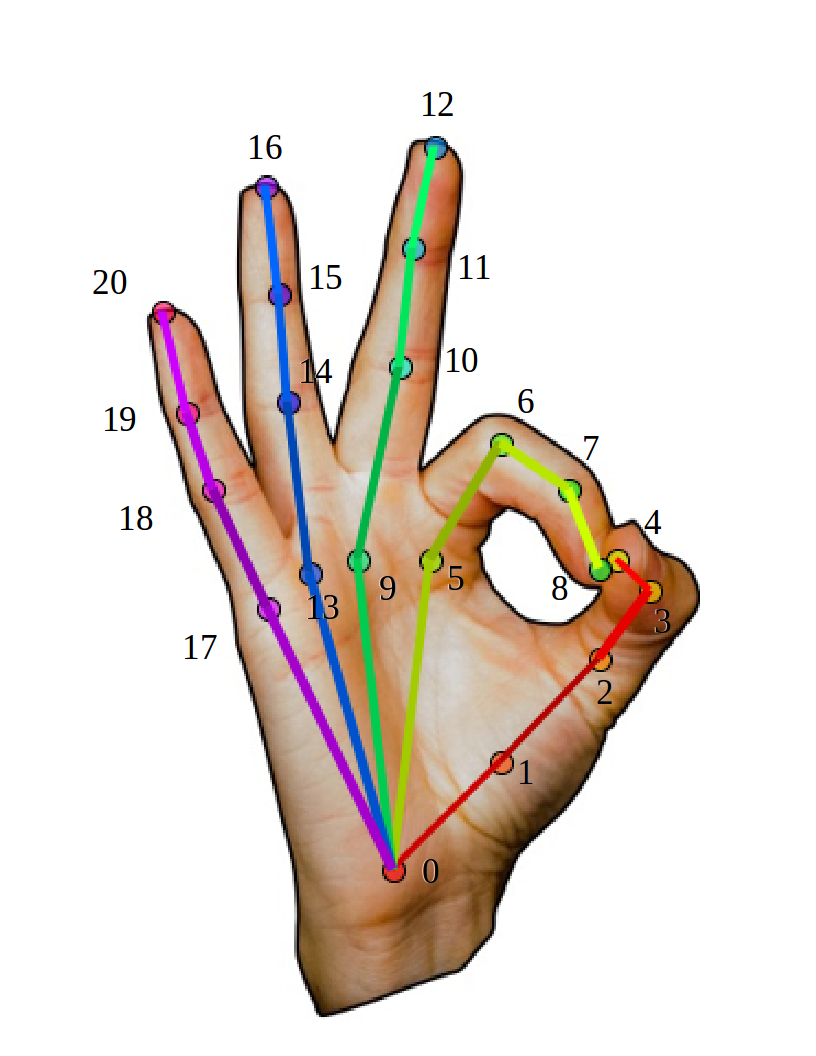
\includegraphics[width=3cm]{images/keypoints_hand}
    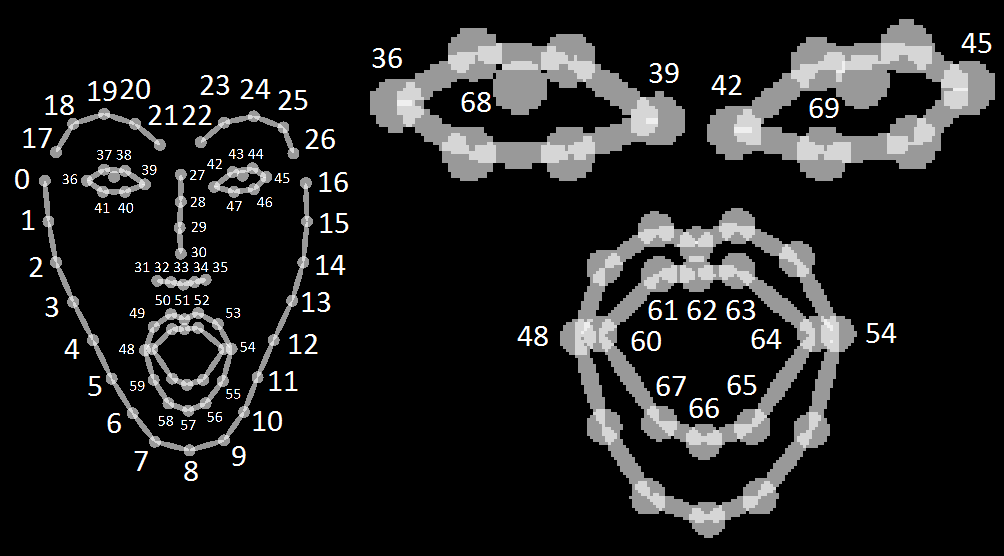
\includegraphics[width=5cm]{images/keypoints_face}
    \caption{Representação dos 21 pontos da mão (à esquerda) e 70 pontos da face (à direita), extraídos pelo OpenPose. Fonte: \cite{openpose-output-2018}.}
    \label{fig:keypoints-face-hand}
\end{figure}

\image
    [5cm]
    {fig:openpose-coordinates}
    {images/openpose_coordinates}
    {Exemplo de arquivo JSON contendo as informações estimadas pelo OpenPose para cada \textit{frame} de vídeo. Cada linha corresponde a um ponto e as colunas referem-se respectivamente, da esquerda para a direita, às coordenadas do eixo X, coordenadas do eixo Y e grau de confiança da estimativa para o par de coordenadas. Fonte: OpenPose.}

A \refimage{fig:sign-pose} ilustra a reconstrução em uma imagem 2D do resultado da estimativa de coordenadas pelo OpenPose para o sinal "EXAGGERATE", bem como a sobreposição dela no vídeo original.

\begin{figure}[ht]
    \centering
    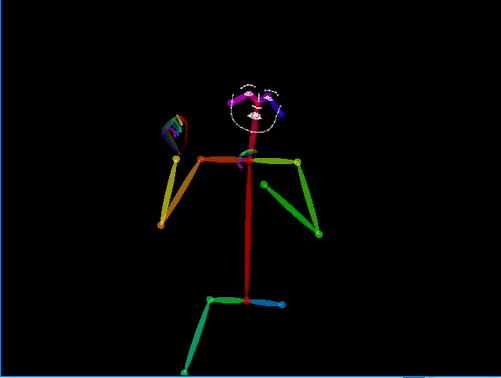
\includegraphics[width=5cm]{images/sign_pose}
    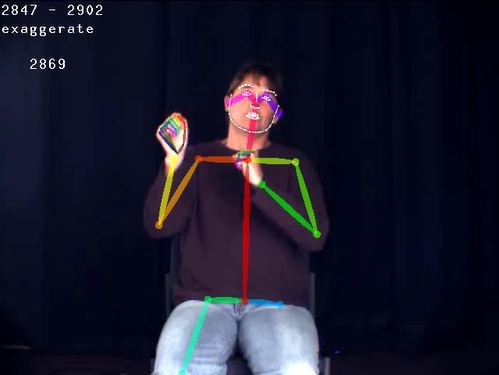
\includegraphics[width=5cm]{images/sign_pose_blended}
    \caption{Reconstrução do esqueleto a partir das coordenadas estimadas pelo OpenPose para um \textit{frame} do sinal "EXAGGERATE" (acima); e sobreposição desse esqueleto no vídeo original (abaixo). Fonte: OpenPose.}
    \label{fig:sign-pose}
\end{figure}

A quarta etapa diz respeito à \textbf{divisão do \textit{dataset}} pré-processado até aqui em subconjuntos que serão utilizados para o treinamento, validação e testes do modelo. Para esse procedimento, foi utilizada uma ferramenta de divisão de \textit{datasets} para validação cruzada disponibilizada pela biblioteca Scikit-Learn \cite{scikit-learn}, denominada "\textit{train\_test\_split}". Por meio dela, primeiramente é subtraída do conjunto original a proporção de amostras destinadas a testes; em seguida, aquelas destinadas à validação; e, por fim, as amostras restantes são destinadas para treinamento. Essa divisão segue como referência a configuração estabelecida a seguir:

\begin{itemize}
    \item 70\% para treinamento;
    \item 15\% para validação;
    \item 15\% para testes.
\end{itemize}

Por fim, a quinta etapa consiste em \textbf{normalizar e serializar} as amostras afim de torná-las compatíveis com o formato de leitura do ST-GCN. A normalização objetiva tornar o comprimento de todas as amostras uniforme, aplicando para isso a repetição de seus \textit{frames} de forma sequencial até o preenchimento completo de um número fixo estabelecido de \textit{frames}. Neste trabalho, o número de \textit{frames} é fixado em 126 (que a uma taxa de 30 FPS, corresponderia a um vídeo de duração aproximada de 4 segundos). A serialização, por sua vez, consiste em pré-carregar as amostras dos subconjuntos criados acima para traduzi-las em arquivos físicos do Python \cite{python}, contendo as respectivas representações em memória desses objetos. Esse é o formato de entrada esperado pelo ST-GCN, que é adotado para otimizar o processo de leitura dos dados. Para cada subconjunto acima são criados dois arquivos físicos: um contendo sua lista de amostras; e outro contendo a lista de rótulos para essas amostras. Esse é, portanto, o resultado final obtido a partir das etapas de pré-processamento do ASLLVD.

As saídas de cada etapa e o \textit{dataset} final pré-processado estão disponíveis publicamente\footnote{
    Disponível em \url{http://www.cin.ufpe.br/~cca5/asllvd-poses}
}.

%%%%%%%%%%%%%%%%%%%%%%%%%%%%%%%%%%%%%%%%%%%%%%%%%%%%%%%%%%%%%%%%%%%%%%%%%%%%%%%%%%%%%%%%%%%%%%%%%%%%%%%%%%%%%%%%%%%%

\subsection{ST-GCN para Reconhecimento da Língua de Sinais} %%%%%%%%%%%%%%%%%%%%%%%%%%%%%%%%%%%%%%%%%%%%%%%%%%%%%%%%%%%%%%%%%%%%%%%%%%%

Conforme comentado acima, foram realizadas adaptações pontuais no código fonte do ST-GCN, mas que não alteram sua arquitetura ou funcionamento essencial. A primeira delas diz respeito à criação de uma nova representação de grafo para o problema da língua de sinais, uma vez que neste trabalho será utilizado um número bem maior de articulações, que vão além daqueles utilizados no trabalho original. Isso se faz necessário para que o modelo seja capaz de compreender os novos pontos do esqueleto e as relações (ou vértices) existentes entre eles. 

De forma análoga a essa necessidade, a outra modificação foi aplicada ao mecanismo de leitura dos dados em \textit{batch} para que ele seja capaz de compreender e aplicar eventuais transformações às matrizes maiores de articulações dos esqueletos que agora estão sendo utilizadas. 

O código fonte contendo as adaptações do ST-GCN aqui apresentadas, bem como a implementação da sequência completa de etapas de pré-processamento está disponibilizado publicamente\footnote{
    Disponível em \url{http://www.cin.ufpe.br/~cca5/st-gcn-sl}
}. Esse código consiste num \textit{fork} criado a partir daquele originalmente desenvolvido pelos autores do modelo.

%%%%%%%%%%%%%%%%%%%%%%%%%%%%%%%%%%%%%%%%%%%%%%%%%%%%%%%%%%%%%%%%%%%%%%%%%%%%%%%%%%%%%%%%%%%%%%%%%%%%%%%%%%%%%%%%%%%%

\section{Resultados} %%%%%%%%%%%%%%%%%%%%%%%%%%%%%%%%%%%%%%%%%%%
\label{sec:resultados}

% Esta seção apresenta as descobertas e resultados obtidos a partir da aplicação da abordagem descrita nas seções anteriores. Os experimentos aqui relacionados foram realizados utilizando uma máquina virtual com CPU Intel Haswell, memória RAM de 5GB e GPU NVIDIA Tesla P100 com 16GB de memória dedicada. O tempo médio obtido com essa arquitetura foi de aproximadamente 7 épocas para cada hora de treinamento.
% O tempo médio consumido para essa tarefa é proporcional ao número de épocas configuradas e tem variado entre 1 e 4 dias

%- configuração máquina

Para este trabalho foram utilizados como referência os experimentos apresentados em \cite{lim-2016} utilizando o ASLLVD (vide \refsect{sec:trabalhos-relacionados}) juntamente com a técnica BHOF. 

Nesses experimentos, os autores utilizaram um subconjunto contendo 20 sinais selecionados a partir do ASLLVD, os quais estão apresentados na \reftable{tab:asllvd-20}. Para reproduzir essa configuração, primeiramente foram utilizadas as poses estimadas no mesmo \textit{dataset} pré-processado na \refsect{sec:experimentos}. A partir dele, foram selecionados os 20 sinais

foram selecionadas as poses estimadas para esses sinais no \textit{dataset} pré-processado na \refsect{sec:experimentos}. Em seguida, foram repetidos os passos de "divisão do \textit{dataset}" e de "normalização e serialização" para que fossem gerados os arquivos de entrada para o modelo considerando apenas as 185 poses referentes a esses sinais, utilizando o mesmo processo descrito na \refsect{sec:experimentos}. O \textit{dataset} final contendo os 20 sinais pré-processados e utilizados neste experimento está disponível publicamente\footnote{
    Disponível em \url{http://www.cin.ufpe.br/~cca5/asllvd-poses-20}
}.

\begin{table}[]
\caption{Sinais selecionados para os experimentos, conforme \cite{lim-2016}}
\label{tab:asllvd-20}
\begin{tabular}{ll}
\hline
Dataset & Isolated Signs \\ \hline
ASLLVD & \begin{tabular}[c]{@{}l@{}}adopt, again, all, awkward, baseball, behavior, can, chat, \\ cheap, cheat, church, coat, conflict, court, deposit, depressed, \\ doctor, don’t want, dress, enough\end{tabular} \\ \hline
\end{tabular}
\end{table}


%- parametros
%Foram considerados \textit{batches} de 32 amostras e uma taxa de aprendizado de 0,1, além de um \textit{weight decay} de 0,0001 em quatro momentos distintos do treinamento (geralmente distribuídos após a conclusão de 35\%, 50\%, 65\% e 80\% das épocas previstas, respectivamente). 
%Adicionalmente, uma estratégia de \textit{data augmentation} para diversificar as amostras apresentadas ao modelo, e ela consiste na aplicação de transformações randômicas de rotação, translação e escala no momento da leitura desses itens nos \textit{batches}.


Para fins de comparação, além do BHOF, os experimentos em \cite{lim-2016} incluem outros métodos populares que foram aplicados sob o mesmo \textit{dataset} de 20 sinais do ASLLVD, como MEI, MHI, PCA, COV e HOF. Os resultados desses métodos também foram reproduzidos na \reftable{tab:results} para que sejam tomados como referência.

%For purposes of comparison, the experiments will include other popular methods such as motion energy image (MEI) [35], motion history image (MHI) [41], principal component analysis (PCA) [42], feature covariance matrix (COV) [30], and histogram of optical flow. The graphical illustration of isolated sign language gesture of MEI, MHI and PCA is shown in Fig. 6. The recognition rates are presented in Table 3. Computation time for each method in frame per seconds (FPS) is shown in the last row of the table. From the results shown, the BHOF method is clearly superior


\begin{table}[ht]
\centering
\caption{My caption}
\label{tab:results}
\begin{tabular}{@{}llllllll@{}}
\toprule
\multirow{2}{*}{Dataset} & \multicolumn{6}{l}{Recognition accuracy (\%)}                                                                \\ \cmidrule(l){2-8} 
            & MEI   & MHI   & PCA   & COV   & HOF   & BHOF   & \textbf{ST-GCN}  \\ \midrule
    ASLLVD  & 25.00 & 10.00 & 45.00 & 45.00 & 70.00 & 85.00  & \textbf{42.86} \\ \bottomrule
\end{tabular}
\end{table}


%- discussão







% A \reftable{tab:resultados-1} apresenta os resultados parciais obtidos da abordagem proposta neste trabalho (representado como ST-GCN (Sign Language), e aqueles obtidos pelo modelo ST-GCN em \cite{st-gcn-2018} (para os \textit{datasets} Kinetics e Kinetics Motion). O resultado do ST-GCN (Sign Language) está listado para o seu treinamento até a época 630 de um total de 1.000 previstas.

% \begin{table}[ht]
%     \centering
%     \caption{Performance atual da abordagem proposta e do ST-GCN original}
%     \label{tab:resultados-1}
%     \begin{tabular}{@{}lll@{}} \toprule
%                                         &   Top-1           &   Top-5           \\ \midrule
%         ST-GCN (Kinetics)               &   30,7\%          &   52,8\%          \\
%         ST-GCN (Kinetics Motion)        &   72,4\%          &   -               \\ \midrule
%         \textbf{ST-GCN (Sign Language)} & \textbf{26,0\%}   &   \textbf{45,2\%} \\ \bottomrule
%     \end{tabular}
% \end{table}

% De acordo com os autores em \cite{st-gcn-2018}, os \textit{datasets} Kinetics e Kinetics Motion diferem-se essencialmente pelo fato de que o primeiro corresponde ao conjunto completo de ações de múltiplos indivíduos (e que muitas vezes incluem a interação desses indivíduos com objetos e com o ambiente à sua volta, que devem ser considerados para classificar tais ações); já o segundo, por sua vez, diz respeito a um subconjunto criado pelos autores para englobar apenas ações descritas exclusivamente pelo movimento dos indivíduos, sem interação com o mundo à sua volta. 

% O motivo disso, nos remete a recapitular a abordagem do ST-GCN de mapear o corpo humano e seus movimentos através de grafos. Ao mesmo tempo em que permite uma observação praticamente completa do esqueleto dos indivíduos, ela abre mão de todos os detalhes adicionais presentes nas cenas em que esses indivíduos estão inseridos. 

% Para o contexto do problema apresentado neste trabalho, entretanto, não há prejuízos decorrentes da não observância dos detalhes da cena, conforme acima. Isso porque nas línguas de sinais o foco é estritamente voltado para o movimento do corpo dos indivíduos (principalmente de partes como mãos, tronco e face), e não é comum que haja interação com objetos durante a articulação dos sinais, mas apenas do corpo com o próprio corpo.



% TODO: incluir gráfico de evolução no treinamento




% Bibliografia
\bibliographystyle{IEEEtran}
\bibliography{IEEEabrv,references.bib}

\end{document}
%%